\section{Lineární přístup}

Většina dnes psaných dokumentů vzniká stále stejným způsobem jako posledních pár století, ani moderní technologie tento přístup moc nezměnili.
Dokumenty vznikají lineárně, nejdříve se vytvoří návrh také nazývaný jako draft, který se poté dá ke kontrole dalším editorům. Ti se zaměří
na jednotlivé části tvořící dokument, kontroluje se pravopis, stylistika a obsah.

Po všech kontrolách se dokument ještě může vrátit autorovi ke konečné kontrole či korekci. Dále poté putuje nakladateli, který dokument,
knihu či odbornou publikaci distribuje. Celý tento postup je znázorněn na grafu pod textem.

Z diagramu je patrné, že jakýkoliv moderní systém pro správu dokumentů, by měl myslet na možnosti jednoduchého sdílení dat mezi autory, korektory a dalšími
subjekty. Aplikace tak nemusí být čistě oreintována na autory, ale měla by nabízet možnost komentovat jednotlivé části dokumentu. Také by měla mít možnost
nabízet data pouze pro čtení, aby nedošlo k chybám a pokud už k nějakým dojde, měla by existovat možnost vrátit se v historii zpět.

V neposlední řadě také musíme myslet na formát výstupu našeho programu, program musí podporovat vícero formátů, aby bylo možné jej šířit na více platformách
a tudíž bylo jej možné dostat vždy ke koncovému uživateli ve formě, kterou může bez potíží otevřít a přečíst.

\clearpage
\begin{center}
    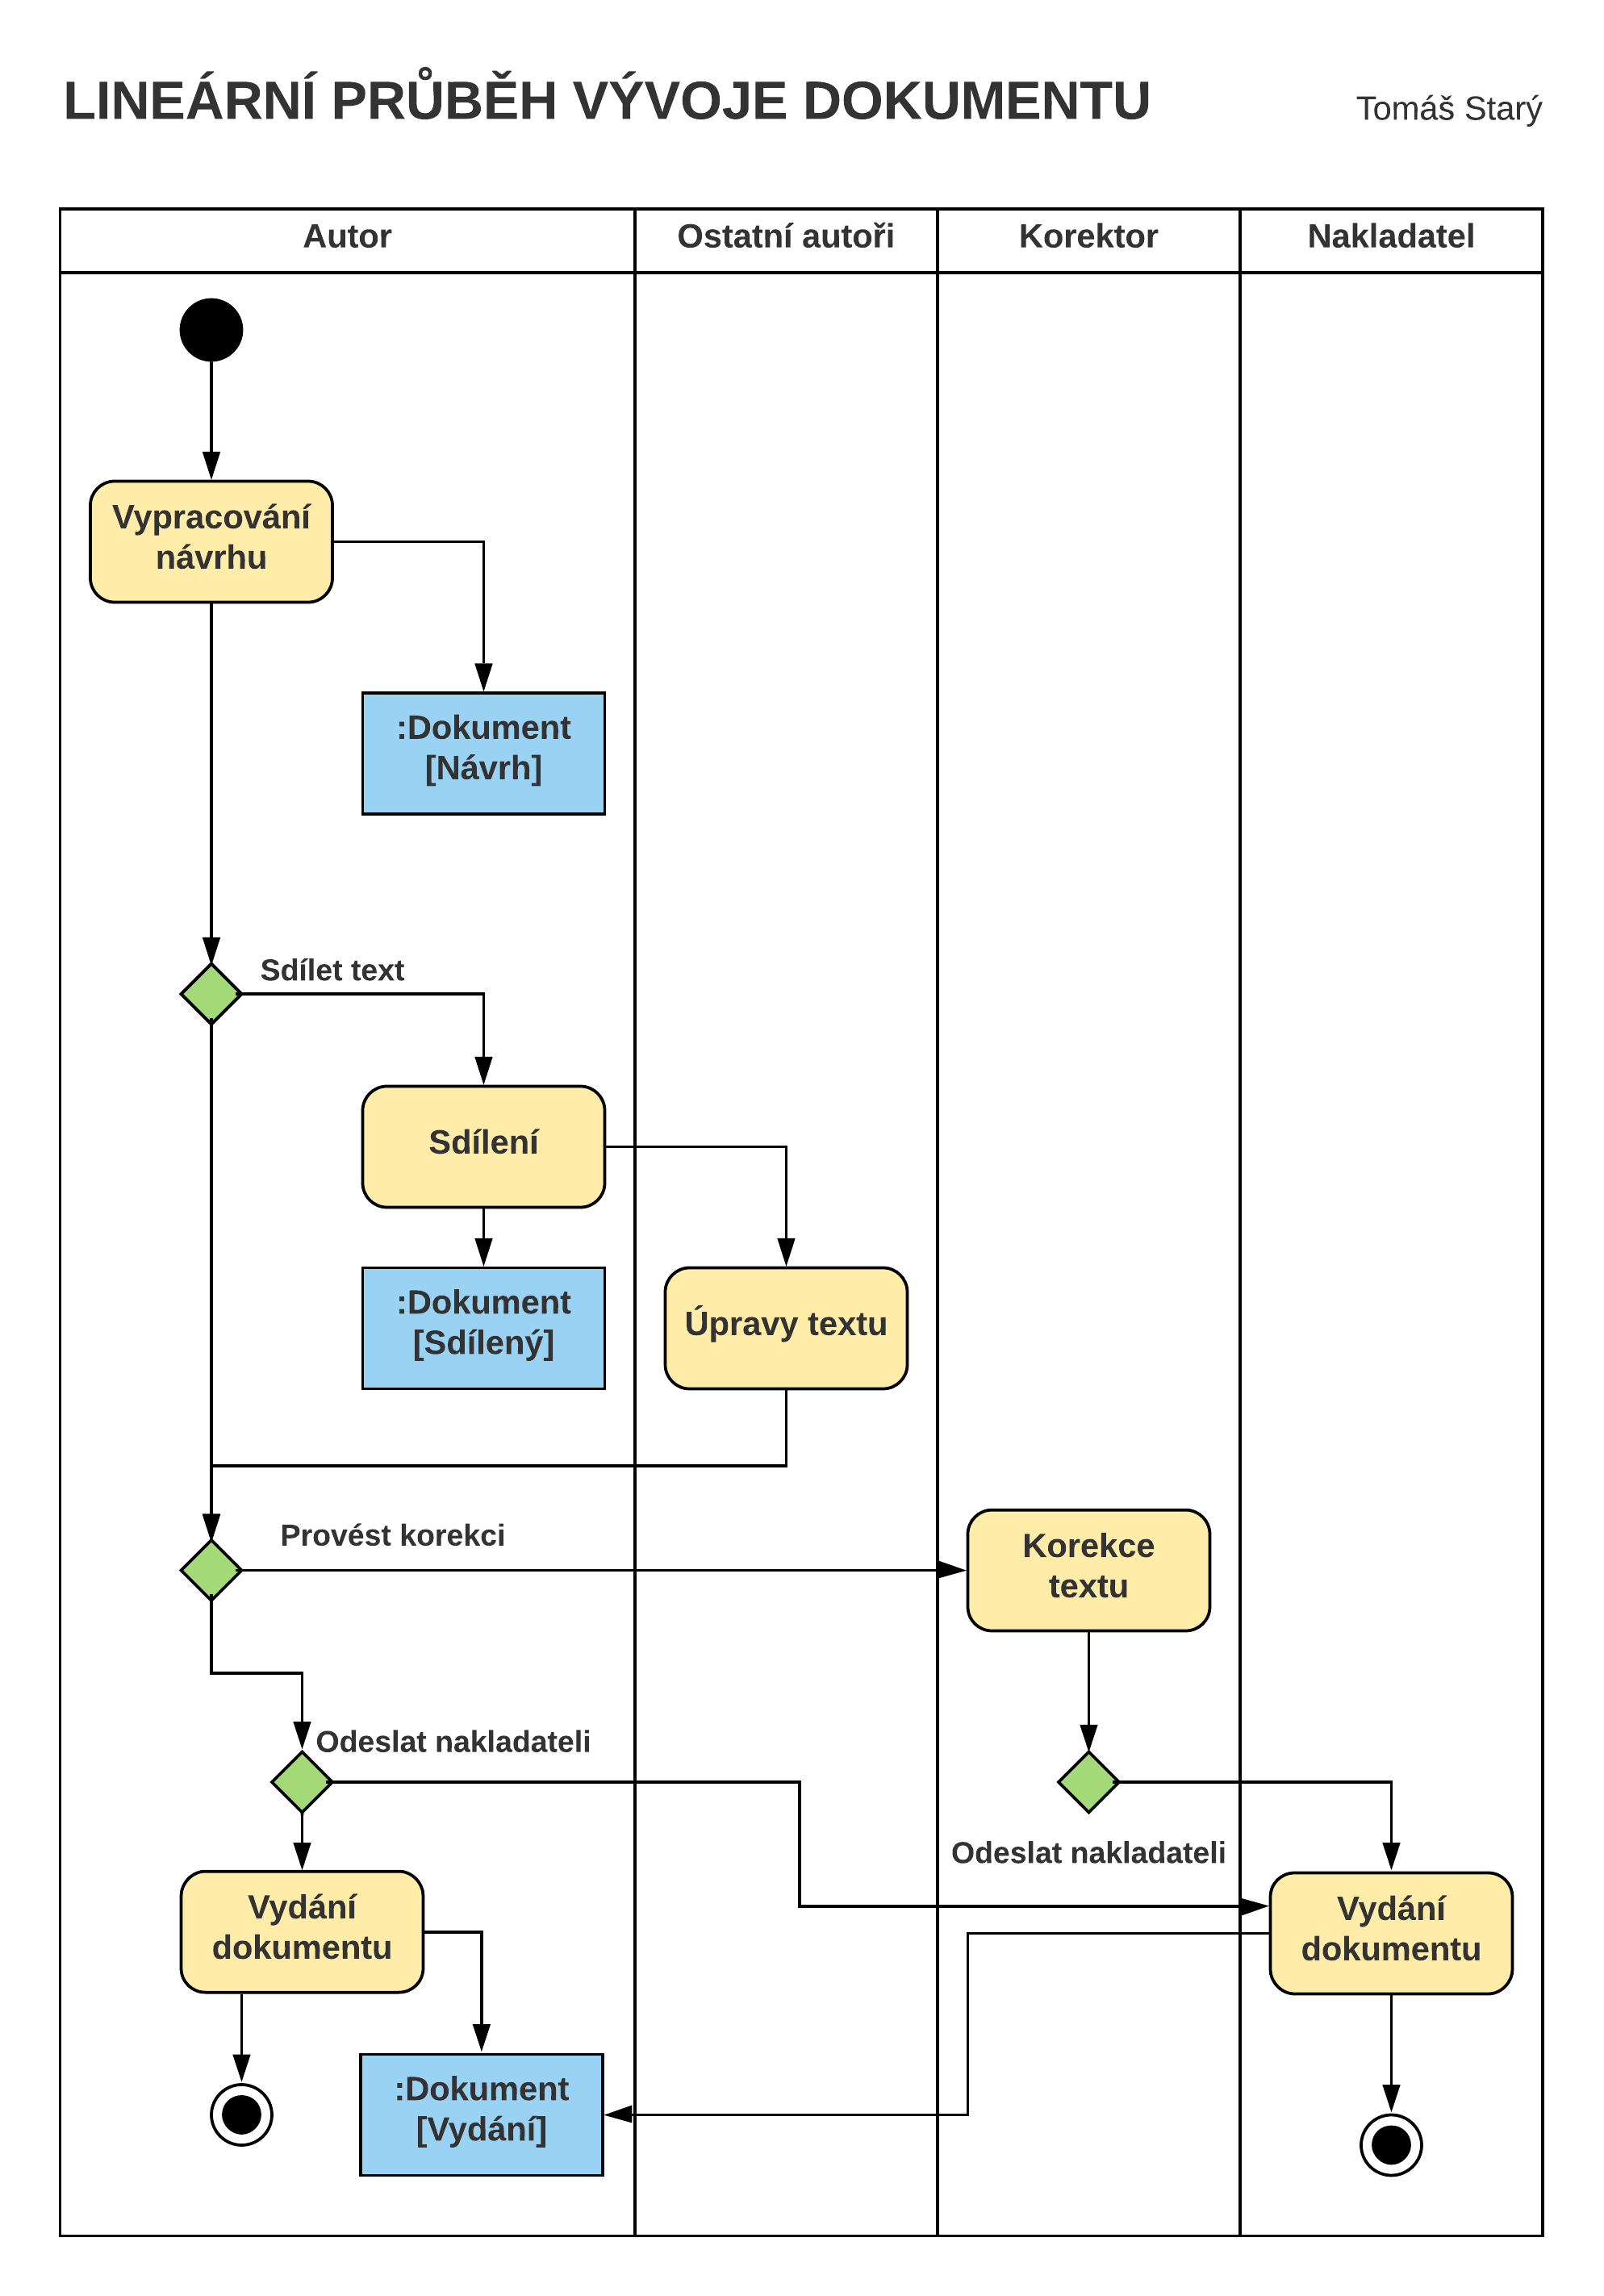
\includegraphics[width=\textwidth]{linearni_prubeh.png}
\end{center}

\section{Modulární přístup}

Modulární přístup k psaní dokumentů je zaměřen na rozdělení dokumentů na jednotlivé moduly, které tvoří dokument. Jako celek si například můžeme představit tuto sekci
textu, nebo i odstavec textu, pokud je logické, že by tato granulita měla smysl. Mezi výhody tohoto rozdělení patří znovupoužtelnost textu mezi více dokumenty, což jistě ocení
lidé, kteří často používají definice, citace či jiné, často se opakující části textu, který je shodný pro více dokumentů.

Jako příklad takového to využití bych viděl v učebních materiálech, sposta definic je stejných a pokud se mají tvořit materiály v podobě nějakých výpisek na cvičení a přednášku,
budou se dané definice opakovat. Pokud ale v dané definici objevím chybu a píšu dokumenty lineárně, musím tuto chybu opravit ve všech dokumentech. V případě modulárních dokumentů
bude pouze stačit opravit definici na jednom místě a změna se promítne ve všech dokumentech. Tímto se také vytvoří nová revize daného dokumentu, takže bude možné jednoduše
sledovat změny nejenom v daném modulu, ale i v dokumentu jako celku.
